%%%%%%%%%%%%%%%%%%%%%%%%%%%%%%%%%%%%%%%%%%%%%%%%%%%%%%%%%%%%%
%% HEADER
%%%%%%%%%%%%%%%%%%%%%%%%%%%%%%%%%%%%%%%%%%%%%%%%%%%%%%%%%%%%%
\documentclass[a4paper,oneside,10pt]{article}

%% ZOTERO bibliography on windows partition

%% Language %%%%%%%%%%%%%%%%%%%%%%%%%%%%%%%%%%%%%%%%%%%%%%%%%
\usepackage[USenglish]{babel} %francais, polish, spanish, ...
\usepackage[T1]{fontenc}
\usepackage[ansinew]{inputenc}
\usepackage[section]{placeins}

\usepackage{lmodern} %Type1-font for non-english texts and characters


%% Packages for Graphics & Figures %%%%%%%%%%%%%%%%%%%%%%%%%%
\usepackage{graphicx} %%For loading graphic files
%\usepackage{subfig} %%Subfigures inside a figure
%\usepackage{pst-all} %%PSTricks - not useable with pdfLaTeX
\usepackage{longtable}
\usepackage{multirow}


%% Math Packages %%%%%%%%%%%%%%%%%%%%%%%%%%%%%%%%%%%%%%%%%%%%
\usepackage{amsmath}
\usepackage{amsthm}
\usepackage{amsfonts}


%%%%%%%%%%%%%%%%%%%%%%%%%%%%%%%%%%%%%%%%%%%%%%%%%%%%%%%%%%%%%
%% DOCUMENT
%%%%%%%%%%%%%%%%%%%%%%%%%%%%%%%%%%%%%%%%%%%%%%%%%%%%%%%%%%%%%
\begin{document}

\pagestyle{empty} %No headings for the first pages.


%% Title Page %%%%%%%%%%%%%%%%%%%%%%%%%%%%%%%%%%%%%%%%%%%%%%%
\title{Predicting League of Legends Match Winner}
\author{Adrien de Castro\\
        Martin le Blanc, \\
        Ausra Pogozelskyte
        }

%\date{} %%If commented, the current date is used.
\maketitle
\begin{abstract}
League of Legends is a popular computer game in which two teams of 5 players faces each other on a battlefield. The publisher of the game, Riot Games, has allowed the public to download match data via an API. These datasets consists of a collection of statistics about matches, such as amount of ressources collected, or number of kills on the enemy. This article will discuss methods of predicting the winner of matches using these datasets.
\end{abstract}

%\tableofcontents %Table of contents
\clearpage

\pagestyle{plain} %Now display headings: headings / fancy / ...

\section{Quick explanation of the game}
\begin{figure}[h]
    \centering
    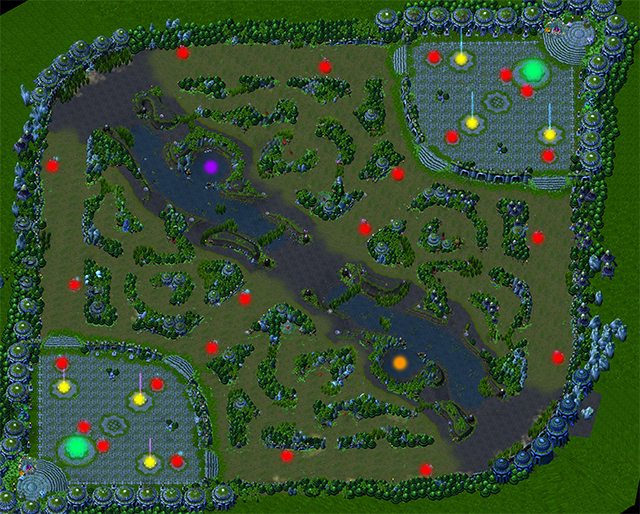
\includegraphics[scale =0.55]{Map.jpg}
    \caption{Summoners Rift Map (\#ref for source-Polygon)}
    \label{fig:map}
\end{figure}

Two teams of five players (a blue and a red one) face each other on a battlefield (cf. fig.\ref{fig:map}). Each player plays a champion. The goal is to destroy the other teams Nexus (in green on the map). There are three lanes (top, middle, bottom). Special roles play in particular lanes (cf. "role" in table \ref{tab:players.dt}). The goal of the first round is to destroy the three opponents towers (the three dots per lane between the river and the base). When players on some lane manage to destroy the three towers, they move to help other players on other lanes or begin destroying the inhibitors (in yellow on the map). When all inhibitors and all towers on the lanes are destroyed, the players can move on to destroying the two towers before the Nexus and eventually destroying it, thus winning the game.

The characters become stronger by buying items (with gold) or by levelling up (with experience). Gold and experience can be won by killing enemies, monsters, minions, completing objectives (?), destroying towers, inhibitors.

For further details we refer you to variable descriptions (tables \ref{tab:players.dt}, \ref{tab:teams.dt}, \ref{tab:match.dt}, \ref{tab:teambans.dt} and \ref{tab:teamstats.dt}) and to \#ref-Polygon.

\section{Dataset}


\begin{longtable}{|c|c|l|}
        \caption{players.dt (1834517x63) (participants + stats1 + stats2)}
        \label{tab:players.dt} \\
        
        % Premier header
        %\toprule
        \hline
        Variable & Type & Description\\
        \hline
        \endfirsthead
        
        %header des pages continues
        %\midrule
        %\endfirsthead
        \multicolumn{3}{l}{\footnotesize\itshape\tablename~\thetable: continued from previous page}\\
        \hline
        Variable & Type & Description\\
        \hline
        \endhead 
        
        % foot des pages continues
        %\midrule
        \multicolumn{3}{r}{\footnotesize\itshape\tablename~\thetable: Continued on next page} \\
        \endfoot
        
        % foot de la dernière page.
        %\midrule
        \multicolumn{3}{r}{\footnotesize\itshape\tablename~\thetable: End} \\
        \endlastfoot
        
        % CONTENU
        \hline
        id                          & scalar          & id used to merge participants, stats1, stats2 \\
        matchid                     & scalar          & Id of the match \\
        player                      & scalar          & Blue team : 1-5, Reg team : 6-10 \\
        championid                  & scalar          & Id of the champion \\
        ss1                         & scalar          & choice of summoner spell 1 \\   
        ss2                         & scalar          & choice of summoner spell 2\\
        role                        & string          & SOLO (mid, top), NONE (jungle),\\ 
        & & DUO\_CARRY/DUO\_SUPPORT (bot)\\
        position                    & string          & bot/jungle/top/mid\\
        win                         & boolean         & if winner \\
        item1                       & scalar          & item 1 in inventory\\
        item2                       & scalar          & item 2 in inventory\\
        item3                       & scalar          & item 3 in inventory\\
        item4                       & scalar          & item 4 in inventory\\
        item5                       & scalar          & item 5 in inventory\\
        item6                       & scalar          & item 6 in inventory\\
        trinket                     & scalar          & free item chosen at the beginning of the match \\
        kills                       & scalar          & number of kills \\
        deaths                      & scalar          & number of deaths \\
        assists                     & scalar          & number of assists \\
        largestkillingspree         & scalar          & number of kills before dying\\
        largestmultikill            & scalar          & nb. tués sans se faire mal ? \\
        killingsprees               & scalar          & number of kills without dying\\
        longesttimespentliving      & scalar          & time spent before dying\\
        doublekills                 & scalar          & number of doublekills\\
        triplekills                 & scalar          & number of triplekills\\
        quadrakills                 & scalar          & number of quadrakills\\
        pentakills                  & scalar          & number of pentakills\\
        legendarykills              & scalar          & number of >penta kills \\
        totdmgdealt                 & scalar          & physical, magical and true damage\\
        magicdmgdealt               & scalar          & magical damage dealt (reduced by "magic spells")\\
        physicaldmgdealt            & scalar          & physical damage dealt (reduced by armour)\\
        truedmgdealt                & scalar          & true damage dealt \footnote{cannot be reduced neither by magical spells nor armour}\\
        largestcrit                 & scalar		  & largest critical strike \footnote{items increase chances of getting critical hits}\\
        totdmgtochamp               & scalar          & total damage dealt to adversary champions\\
        magicdmgtochamp             & scalar          & magical damage dealt to adversary champions\\
        physdmgtochamp              & scalar          & physical damage dealt to adversary champion\\
        truedmgtochamp              & scalar          & true damage dealt to adversary champion\\
        totheal                     & scalar          & total healed damage\\
        totunitshealed              & scalar          & number of characters \footnote{player or NPC (non-player character)}\\
        dmgselfmit                  & scalar          & damage prevented using armour or magic spells\\
        dmgtoobj                    & scalar          & damage to objectives\\
        dmgtoturrets                & scalar          & damage to turrets\\
        visionscore                 & scalar          & ??\\
        timecc                      & scalar          & Time spent  crowd control \footnote{healers have high timecc}\\
        totdmgtaken                 & scalar          & total damage taken\\
        magicdmgtaken               & scalar          & magic damage taken\\
        physdmgtaken                & scalar          & physical damage taken\\
        truedmgtaken                & scalar          & true damage taken\\
        goldearned                  & scalar          & gold earned\\
        goldspent                   & scalar          & gold spent\\
        turretkills                 & scalar          & number of turrets destoyed\\
        inhibkills                  & scalar          & number of inhibitors destroyed\\
        totminionskilled            & scalar          & number of minions killed\\
        neutralminionskilled        & scalar          & number of neutral minions killed\\
        ownjunglekills              & scalar          & ???\\
        enemyjunglekills            & scalar          & nb. des minions ennemis \\
        totcctimedealt              & scalar          & ? diff ac. timecc"\\
        champlvl                    & scalar          & level of the champion\\
        pinksbought                 & scalar          & Number of pinks \footnote{special ward that enables players to see invisible wards}  bought\\
        wardsbought                 & scalar          & wards bought (compté comment ?)\\
        wardsplaced                 & scalar          & wards placed\\
        wardskilled                 & scalar          & wards destroyed\\
        firstblood                  & boolean         & if player had first kill \\
        \hline
\end{longtable}
\newpage

\begin{longtable}{|c|c|l|}
        \caption{teams.dt (345268x58)}
        \label{tab:teams.dt} \\
        
        % Premier header
        %\toprule
        \hline
        Variable & Type & Description\\
        \hline
        \endfirsthead
        
        %header des pages continues
        %\midrule
        %\endfirsthead
        \multicolumn{3}{l}{\footnotesize\itshape\tablename~\thetable: continued from previous page}\\
        \hline
        Variable & Type & Description\\
        \hline
        \endhead 
        
        % foot des pages continues
        %\midrule
        \multicolumn{3}{r}{\footnotesize\itshape\tablename~\thetable: Continued on next page} \\
        \endfoot
        
        % foot de la dernière page.
        %\midrule
        \multicolumn{3}{r}{\footnotesize\itshape\tablename~\thetable: End} \\
        \endlastfoot
        
        % CONTENU
        \hline
        matchid                     & scalar          & Id of the match \\
        teamid                      & scalar          & Blue team : 100, Reg team : 200 \\
        firstblood                  & boolean         & if the team had the first kill\\
        firsttower                  & boolean         & first to destroy a tower \\
        firstinhib                  & boolean         & first to destroy an inhibitator \\
        firstbaron                  & boolean         & first to kill a baron \\
        firstdragon                 & boolean         & first to kill a dragon \\
        firstharry                  & boolean         & first to kill a harry \\
        towerkills                  & scalar          & number of towers destroyed\\
        inhibkills                  & scalar          & number of inhibitors destroyed\\
        baronkills                  & scalar          & number of barons killed\\
        dragonkills                 & scalar          & number of dragons killed\\
        harrykills                  & scalar          & number of harrys killed\\
        duration                    & scalar          & duration in seconds of the match\\
        win                         & boolean         & if winner \\
        kills                       & scalar          & sum of kills per player\\
        deaths                      & scalar          & sum of deaths per player\\
        assists                     & scalar          & sum of assists per player\\
        
        largestkillingspree         & scalar          & number of kills before dying\\
        largestmultikill            & scalar          & nb. tués sans se faire mal ? \\
        killingsprees               & scalar          & number of kills without dying\\
        longesttimespentliving      & scalar          & time spent before dying\\
        doublekills                 & scalar          & number of doublekills\\
        triplekills                 & scalar          & number of triplekills\\
        quadrakills                 & scalar          & number of quadrakills\\
        pentakills                  & scalar          & number of pentakills\\
        legendarykills              & scalar          & number of >penta kills \\
        totdmgdealt                 & scalar          & physical, magical and true damage\\
        magicdmgdealt               & scalar          & magical damage dealt (reduced by "magic spells")\\
        physicaldmgdealt            & scalar          & physical damage dealt (reduced by armour)\\
        truedmgdealt                & scalar          & true damage dealt \footnote{cannot be reduced neither by magical spells nor armour}\\
        largestcrit                 & scalar		  & largest critical strike \footnote{items increase chances of getting critical hits}\\
        totdmgtochamp               & scalar          & total damage dealt to adversary champions\\
        magicdmgtochamp             & scalar          & magical damage dealt to adversary champions\\
        physdmgtochamp              & scalar          & physical damage dealt to adversary champion\\
        truedmgtochamp              & scalar          & true damage dealt to adversary champion\\
        totheal                     & scalar          & total healed damage\\
        totunitshealed              & scalar          & number of characters \footnote{player or NPC (non-player character)}\\
        dmgselfmit                  & scalar          & damage prevented using armour or magic spells\\
        dmgtoobj                    & scalar          & damage to objectives\\
        dmgtoturrets                & scalar          & damage to turrets\\
        visionscore                 & scalar          & ??\\
        totdmgtaken                 & scalar          & total damage taken\\
        magicdmgtaken               & scalar          & magic damage taken\\
        physdmgtaken                & scalar          & physical damage taken\\
        truedmgtaken                & scalar          & true damage taken\\
        goldearned                  & scalar          & gold earned\\
        goldspent                   & scalar          & gold spent\\
        (?) turretkills             & scalar          & number of turrets destoyed\\
        (?) inhibkills              & scalar          & number of inhibitors destroyed\\
        totminionskilled            & scalar          & number of minions killed\\
        (?) neutralminionskilled    & scalar          & number of neutral minions killed\\
        ownjunglekills              & scalar          & ???\\
        enemyjunglekills            & scalar          & nb. des minions ennemis \\
        totcctimedealt              & scalar          & ? diff ac. timecc"\\
        maxchamplvl                 & scalar          & level of the champion\\
        avgchamplvl                 & scalar          & \\
        minchamplvl                 & scalar          & \\
        pinksbought                 & scalar          & Number of pinks \footnote{special ward that enables players to see invisible wards}  bought\\
        (?) wardsbought             & scalar          & wards bought (compté comment ?)\\
        wardsplaced                 & scalar          & wards placed\\
        wardskilled                 & scalar          & wards destroyed\\
        \hline
\end{longtable}
\newpage

\begin{longtable}{|c|c|l|}
        \caption{match.dt data (184069x8)}
        \label{tab:match.dt} \\
        
        % Premier header
        %\toprule
        \hline
        Variable & Type & Description\\
        \hline
        \endfirsthead
        
        % CONTENU
        \hline
        id              & scalar        & Id\\
        gameid          & scalar        & match Id\\
        platformid      & string        & server on which the match took place\\
        queueid         & scalar        & ???\\
        seasonid        & scalar        & id of the session\\
        duration        & scalar        & duration in seconds of the match\\
        creation        & scalar        & creation time-stamp in milliseconds\\
        version         & string        & patch of the match\\
        \hline
\end{longtable}

\begin{longtable}{|c|c|l|}
        \caption{teambans.dt data (1099185x4)}
        \label{tab:teambans.dt} \\
        
        % Premier header
        %\toprule
        \hline
        Variable & Type & Description\\
        \hline
        \endfirsthead
        
        % CONTENU
        \hline
        matchid           & scalar          & Id of the match \\
        teamid            & scalar          & Id of the team (100 or 200) \\
        championid        & scalar          & Which champion has been banned \\
        banturn           & scalar          & The turn at which the champion has been banned \footnote{at the beginning of the match, each team take turns to ban three champions each, preventing players from both teams to choose those champions.} \\
        \hline
\end{longtable}

\begin{longtable}{|c|c|l|}
        \caption{teamstats.dt data (368138x13)}
        \label{tab:teamstats.dt} \\
        
        % Premier header
        %\toprule
        \hline
        Variable & Type & Description\\
        \hline
        \endfirsthead
        
        % CONTENU
        \hline
        matchid           & scalar          & Id of the match \\    
        teamid            & scalar          & Id of the team (100 or 200) \\      
        firstblood        & boolean         & first to kill \footnote{player get extra 100 gold}\\
        firsttower        & boolean         & first to destroy a tower \footnote{extra 300 gold spread accross nearby players.} \\
        firstinhib        & boolean         & first to destroy an inhibitor\\
        firstbaron        & boolean         & first to kill a baron \\
        firstdragon       & boolean         & first to kill a dragon \\
        firstharry        & boolean         & first to kill a harry \footnote{}\\
        towerkills        & scalar          & number of towers destroyed \\
        inhibkills        & scalar          & number of inhibitors destroyed \footnote{They respawn five minutes after being destroyed. Releases super-minions when destroyed.} \\
        baronkills        & scalar          & number of barons killed \footnote{In in the figure \ref{fig:map}. Killing a Baron Nasher gives more attack damage, ability power, bonus health and manner regeneration. Killing it gives big advantage in the late game. Gives 300 gold and 600 XP to all players in the team and an additional bonus for the player who killed it.}\\
        dragonkills       & scalar          & number of dragons killed \footnote{it gives the Dragon Slayer buff (exp!). Killing it gives 25 gold and 75-300 gold.} \\
        harrykills        & scalar          & number of harrys killed \\ 
        \hline
\end{longtable}

\end{document}

